\section{Mobile Platforms and the Market}

The demand for applications to be portable on mobile phones and tablets has
become a fashion as well as accessibility on the go. In the current market
cryptic crosswords are available in a variety of newspapers, magazines and
online websites. These are everyday media in which a person can access their
favourite cryptic crosswords and participate in. With the expansion of mobile
phone and tablet applications research has shown that a unique cryptic crossword
solver has not been incorporated in any of the mobile operating systems. There
are applications, which can be downloaded, that contain pre-solved crosswords but there is no real solver, which solves cryptic crosswords in real time. In fact research has shown that there is only a very small handful of cryptic crossword applications across all mobile operating systems.

\subsection{Mobile Operating Systems}

The Oxford English dictionary states an ``Operating System'' as `the low-level
software that supports a computer's basic functions, such as scheduling tasks
and controlling peripherals' \citep{oxford_dictionary11}.

A mobile operating system has the same definition but supports the basic
functions for handheld devices such as mobile phones and tablets. In the current
market the term mobile operating system is associated with smartphones rather
than mobile phones due to the powerful processors, which are embedded in the
mobile phone devices.

The official first mobile operating system for smartphones was by IBM introduced
in 2000 as the `Simon' but it was Ericson who created the first all in one
smartphone with the Symbian OS, which incorporated a keyboard hence, the term
smartphone was introduced. This ran on various mobile phones by companies such
as Ericcson, Samsung but predominantly on smartphones by Nokia. This created a
path for a market, which was to be dominated by others in the coming future
\citep{smartphone11}.

By 2007 from the back of a successful campaign selling music devices known as
the iPod, Apple introduced the Apple iPhone which came with their fist mobile
operating system the iOS which was a full operating system used from the Mac OS
X 10 \citep{macworld07}.

By July 2008 Apple released iOS 2.0 and with this came the application store.
This was a revolution to the mobile market allowing a platform for third party
developers to sell and market their own applications for the mobile operating
system. On the 7th January 2013 Apple announced that they have had more than 40
Billion downloads of applications  through their application store
\citep{40billion12}.

In September 2008 Google released their own version of a mobile operating system
``Android'' which had its similarities of marketing with its very own application store known as the android market which since has been rebranded as the Google play store.

In April 2009 BlackBerry also launched it's own application store called the
BlackBerry World, which works with their mobile operating system the BlackBerry
10 \citep{bbworld09}.

Finally windows released their version of an application store for distribution 
of applications on October 26th 2012 \citep{windows8}.

Although there are now several platforms that run on a mobile device, Android
and iOS combine for 91.1\% of the worldwide smartphone operating system market \citep{idc13}.

This shows that although BlackBerry has been in the market since 2009 there
isn't much of a rise to interests in their applications and while Windows is 
fairly new it has a lot of ground to cover to catch up with their main 
competitors.

For the purpose of this project it is pretty clear to what is demanded from
consumers in the real world with Apple and Google being the two main competitors
for mobile applications. In order to decide on what platform the project will be
suitable for to design, maintain and deploy a good working product the following tables cover some of the reasons which could be
possible to allow the team members to come to a decision to what pathway the
project will be going in.

\begin{table}[H]
  \centering
  \small
  \begin{tabular}{|p{2cm}|p{3cm}|p{2cm}|p{2.5cm}|p{2.5cm}|}
  \hline
  \textbf{Platform} & \textbf{Programming Language} & \textbf{Open Source} &
  \textbf{Open API/SDK} & \textbf{License} \\ \hline
  Android & Java & Yes & Yes & Apache \\ \hline
  iOS & Objective C & N/A & Yes & Proprietary \\ \hline
  BlackBerry & Java, C++ & N/A & Yes & Proprietary \\ \hline
  Windows & C, C++, C\#& N/A & Yes & Microsoft \\ \hline 
  \end{tabular}
  \caption {A comparison of mobile platforms}
\end{table}


\begin{table}[H]
  \centering
  \small
  \begin{tabular}{|p{2cm}|p{3.5cm}|p{2.2cm}|p{4.5cm}|p{2cm}|}
  \hline
  \textbf{Platform} & \textbf{Latest Version} & \textbf{Debugging} &
  \textbf{Hardware / Software Requirements} & \textbf{Emulator} \\ \hline
  Android & 4.3 Jelly Bean & Yes & Windows / Mac & Yes \\ \hline
  iOS & iOS 7 & Yes & Intel Based Mac & Yes  \\ \hline
  BlackBerry & BlackBerry 10 & Yes & Windows / Mac & Yes \\ \hline
  Windows & Windows Phone 8 & Yes & Windows & Yes \\ \hline
  \end{tabular}
  \caption {A further comparison of mobile platforms}
\end{table}

\begin{table}[H]
  \centering
  \small
  \begin{tabular}{|p{2cm}|p{2.2cm}|p{3cm}|p{3cm}|p{4cm}|}
  \hline
  \textbf{Platform} & \textbf{Underlying OS} & \textbf{Development
  Environment} & \textbf{Submission To application Store} & \textbf{Development Cost}
  \\ \hline
  Android & Linux & Eclipse & Unlimited & \$25 One Off cost \\ \hline
  iOS & Darwin & XCode & Unlimited & \pounds60 Yearly / \$99 \\ \hline
  BlackBerry & BlackBerry OS & Eclipse & 100 Per Year & \$100 One off cost
  \\ \hline
  Windows & Windows & Visual Studio & Unlimited & \$19 Yearly / Free for
  Dreamspark Students \\ \hline
  \end{tabular}
  \caption{More comparisons of mobile platforms}
\end{table}

Although these are the four main types of platforms available in the market for
mobile development there is a growing amount of organisations, which are
developing tools to allow developers to create cross platform application with
ease. Two of these are Appcelerator and Adobe AIR.

\begin{table}[H]
  \centering
  \small
  \begin{tabular}{|p{2.5cm}|p{2.7cm}|p{1.8cm}|p{2cm}|p{2.8cm}|p{2.8cm}|}
  \hline
  \textbf{Platform} & \textbf{Programming Language} & \textbf{Open Source} &
  \textbf{Open API/SDK} & \textbf{Underlying OS and License} &
  \textbf{Development Environment} \\ \hline
  Appcelerator & JavaScript & Yes & Yes & Linux Apache 2.0 & Eclipse Based
  IDE / Titanium Studio \\ \hline
  Adobe AIR & ActionScript, HTML, CSS, JavaScript & No & Yes & Darwin
  Proprietary & Adobe AIR \\ \hline
  \end{tabular}
  \caption {A comparison of cross platform development tools}
\end{table}

\newpage
\subsection{Appcelerator}

Appcelerator is a platform created by Appcelerator Inc to allow developers to
create cross platform native applications for Android and iOS. They later
introduced compatibility for BlackBerry 10 and are in the process of developing
for Windows Phone. The main development environment used to create applications
is an Eclipse based IDE known as Titanium Studio. Developers can create great
looking native applications  using JavaScript. The use and license of 
Appcelerator falls under Apache 2.0.

\subsection{Adobe AIR}

Adobe Integrated Runtime (Adobe AIR) uses adobe tools such as flash to allow
developers to create platform independent web applications. Unlike Appcelerator
this means that applications created can only be web based and not native. For
this reason a lot of developers avoid using Adobe AIR. It supports all the major
vendors for mobile applications but applications created in Adobe AIR are a lot
slower.


\newpage
\subsection{Native Applications}

A native application is a platform independent application designed to work with
a particular mobile OS. The application is installed on the device whether it's
a smartphone or a tablet.

Advantages

\begin{itemize}
  \item Faster at accessing device features such as camera and accelerometer
  \item Easy to find in application stores such as Google Play and Apple 
        application store
  \item Secure as they go through an approval phase from vendors
\end{itemize}


Disadvantages

\begin{itemize}
  \item Expensive to develop
  \item Expensive to maintain
  \item Approval process can take from days to months
  \item Support of the application can be hard to maintain due to different 
        people using different versions of operating system installed.
\end{itemize}

\subsection{Web Applications}

A web application is really a website designed to look and feel like an 
application. This is wrapped by the web browser, which means an Internet
connection is required to use the applications. Google Chrome and Safari are 
examples of Web applications.

Advantages

\begin{itemize}
  \item Easy to maintain
  \item Can be compatible with any device
  \item Approval is not required
  \item Easy to maintain and update without affecting the user to update the
  software
\end{itemize}

Disadvantages

\begin{itemize}
  \item Limited to what can be accessed on the devices
  \item Hard to provide support over various Web browsers
  \item Not easy to find and promote, users will have to browse websites
  \item Can be insecure due to the application being web based
\end{itemize}

There are various platforms available for mobile devices. The most popular
platforms are the previously mentioned. Although they are in contest, the use
and popularity of platforms vary from region to region. An article published by
\citet{wpcentral13} states that windows phone is the most popular platform in
Latin America. Although the platform was produced later than the other platforms
this has become popular due to the lower prices of devices. Devices such as the
iPhone and the iPad are a lot dearer and can cost a user a couple of hundred
pounds. In September Forbes reported that the most popular platform on mobile
devices is Android.

\newpage
\begin{figure}[H]
  \centering
  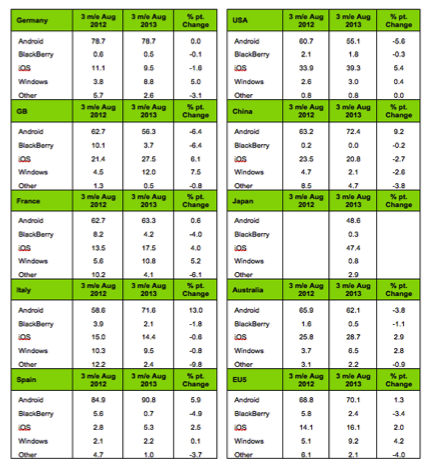
\includegraphics[scale=0.75]{forbeslist13.png}
  \caption{Mobile phone market share September 2013}
\end{figure}

\begin{flushright}
\citep{forbes13}
\end{flushright}

\subsection{Currently available Cryptic Crossword Applications}

After performing various research on the apple application store, the Google
play store and BlackBerry world, it was discovered that there is not many
cryptic crosswords available to download. There were two, which could be clearly
defined as cryptic crossword applications, and these have been analysed in the
following sections.

\subsection{Puzzler Super Cryptic Crosswords}

Platform: Apple iOS \\ 
Price: \pounds3.99 \\ 
Compatibility: iOS 4.3 or Later \\
Website: https://itunes.apple.com/gb/app/puzzler-super-cryptic-crosswords/id616060420?mt=8

\begin{figure}[H]
  \centering
  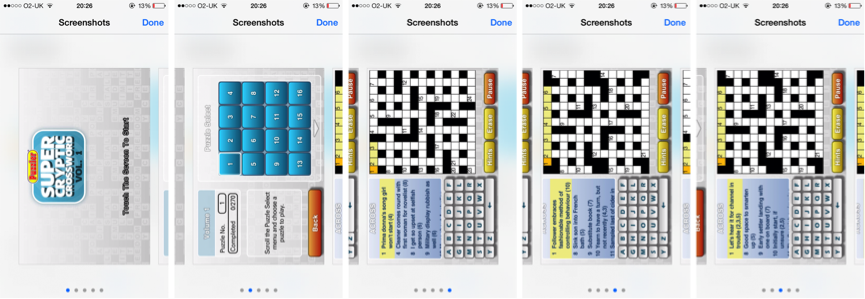
\includegraphics[width=\linewidth]{pscs.png}
  \caption{Screenshots of Puzzler Super Cryptic Crosswords on iPhone}
\end{figure}

This application contains 270 pre built crosswords. The interface is really easy
to use and it clearly shows what has been completed and what needs to be
completed. What's nice about this application is that the crosswords are in
various levels and as you complete one crossword you can move on to the next.
What was noticed is that the application already stores the answers and also the
application allows hints, which makes it a little easier to use. The other
noticeable thing about this application is that it didn't fully use the native
features of the mobile phone. Like the keyboard is a custom keyboard.


\subsection{Cryptic Crossword}

Platform: Apple iOS, Android \\ 
Price: Free with 2 puzzles on Apple devices 
        -- In application purchase available 
        -- \pounds1.99 on Android Devices \\ 
Compatibility: iOS 6.0 or Later \\ 
Website: https://itunes.apple.com/gb/app/cryptic-crossword/id661608021?mt=8


\begin{figure}[H]
  \centering
  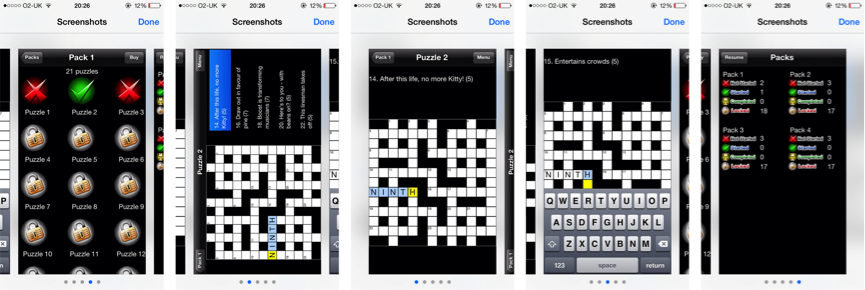
\includegraphics[width=\linewidth]{cc.png}
  \caption{Screenshots of Cryptic Crossword on iPhone}
\end{figure}

The Cryptic Crosswords application comes with 4 different packages and a total
of 81 puzzles. Each pack can be bought for \pounds0.69 or all 4 for a discounted
price of \pounds1.99. Each package contains various cryptic crossword puzzles.
After having a play around with this application at first point of contact it is
noticed that look and feel of the application is not that great. The use of
colours and the layout styles of the application can be better. The application
consists of 81 puzzles, which can be played only after each crossword has been
completed. Some of the features of the application are:

\begin{itemize}
  \item Checking answers
  \item Revealing a letter, a word or the whole puzzle
  \item Clearing the puzzle
  \item Moving the character bar to next box
  \item Greying out completed clues
\end{itemize}

These are some of the features the application uses but there are plenty more.
